\documentclass{article}%
\usepackage[T1]{fontenc}%
\usepackage[utf8]{inputenc}%
\usepackage{lmodern}%
\usepackage{textcomp}%
\usepackage{lastpage}%
\usepackage[head=40pt,margin=0.5in,bottom=0.6in]{geometry}%
\usepackage{graphicx}%
%
\title{\textbf{Reportan presencia de crudo en las costa del oeste de Anzoátegui}}%
\author{MIRIAM RIVERO}%
\date{28/09/2018}%
%
\begin{document}%
\normalsize%
\maketitle%
\textbf{URL: }%
http://www.eluniversal.com/venezuela/21874/reportan{-}presencia{-}de{-}crudo{-}en{-}las{-}costas{-}oeste{-}del{-}estado{-}anzoategui\newline%
%
\textbf{Periodico: }%
EU, %
ID: %
21874, %
Seccion: %
venezuela\newline%
%
\textbf{Palabras Claves: }%
NO\_TIENE\newline%
%
\textbf{Derecho: }%
3.2%
, Otros Derechos: %
NO\_TIENE%
, Sub Derechos: %
3.2.1%
\newline%
%
\textbf{EP: }%
NO\newline%
\newline%
%
\textbf{\textit{Habitantes de los municipios Peñalver y Píritu se encuentran en estado de alarma por el derrame de petróleo que se observa en la orilla de las playas}}%
\newline%
\newline%
%
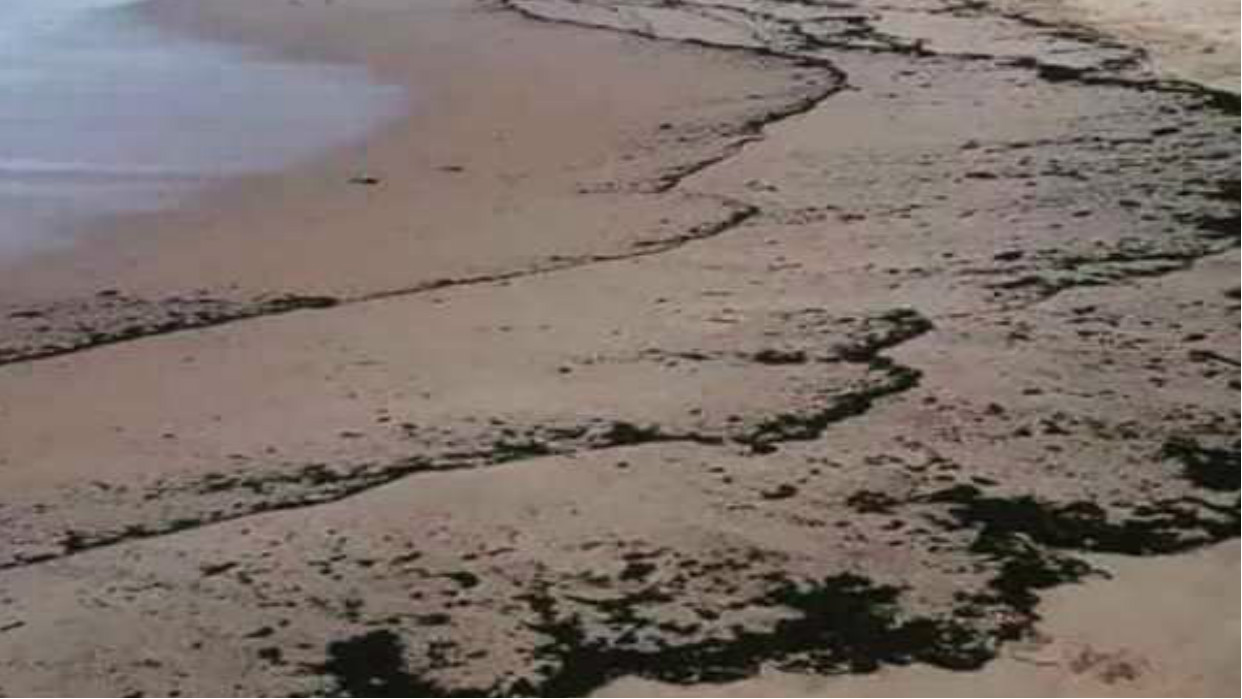
\includegraphics[width=300px]{256.jpg}%
\newline%
%
Aunque no es la primera vez que ocurre esta situación, los moradores están exhortando a las autoridades locales, regionales y petroleras tomar las medidas de saneamiento correspondientes.~Los sectores más afectados son el bulevar Fernández Padilla y la playa La Cerca, donde se observan los residuos de petróleo, según lo informado por el promotor turístico de la entidad, Humberto Guerra, quien señaló que estas zonas son sustentos económicos para muchos residentes.~Según las denuncias tanto de Guerra como de los vecinos afectados, la grave contaminación se viene observando desde el día miércoles; sin embargo, trascendió que el accidente ocurrió el domingo en las instalaciones del Complejo Petrolero José Antonio Anzoátegui.%
\newline%
%
\end{document}